\documentclass[a4paper,11pt]{exam}
\printanswers % pour imprimer les réponses (corrigé)
%\noprintanswers % Pour ne pas imprimer les réponses (énoncé)
\addpoints % Pour compter les points
% \noaddpoints % pour ne pas compter les points
%\qformat{\textbf{\thequestion ) } }
%\qformat{\textbf{\thequestion )} (\thepoints) \\} % Pour définir le style des questions (facultatif)
\usepackage{color} % définit une nouvelle couleur
\shadedsolutions % définit le style des réponses
% \framedsolutions % définit le style des réponses
\definecolor{SolutionColor}{rgb}{0.8,0.9,1} % bleu ciel
\renewcommand{\solutiontitle}{\noindent\textbf{Solution:}\par\noindent} % Définit le titre des solutions




\makeatletter

\def\maketitle{{\centering%
	\par{\huge\textbf{\@title}}%
	\par{\@date}%
	\par}}

\makeatother

\lhead{NOM Pr\'enom :}
\rhead{\textbf{Les r\'eponses doivent \^etre justifi\'ees}}
\cfoot{\thepage / \pageref{LastPage}}


%\usepackage{../../pas-math}
%\usepackage{../../moncours}


%\usepackage{pas-cours}
%-------------------------------------------------------------------------------
%          -Packages nécessaires pour écrire en Français et en UTF8-
%-------------------------------------------------------------------------------
\usepackage[utf8]{inputenc}
\usepackage[frenchb]{babel}
\usepackage[T1]{fontenc}
\usepackage{lmodern}
\usepackage{textcomp}



%-------------------------------------------------------------------------------

%-------------------------------------------------------------------------------
%                          -Outils de mise en forme-
%-------------------------------------------------------------------------------
\usepackage{hyperref}
\hypersetup{pdfstartview=XYZ}
%\usepackage{enumerate}
\usepackage{graphicx}
\usepackage{multicol}
\usepackage{tabularx}
\usepackage{multirow}


\usepackage{anysize} %%pour pouvoir mettre les marges qu'on veut
%\marginsize{2.5cm}{2.5cm}{2.5cm}{2.5cm}

\usepackage{indentfirst} %%pour que les premier paragraphes soient aussi indentés
\usepackage{verbatim}
\usepackage{enumitem}
\usepackage[usenames,dvipsnames,svgnames,table]{xcolor}

\usepackage{variations}

%-------------------------------------------------------------------------------


%-------------------------------------------------------------------------------
%                  -Nécessaires pour écrire des mathématiques-
%-------------------------------------------------------------------------------
\usepackage{amsfonts}
\usepackage{amssymb}
\usepackage{amsmath}
\usepackage{amsthm}
\usepackage{tikz}
\usepackage{xlop}
%-------------------------------------------------------------------------------



%-------------------------------------------------------------------------------


%-------------------------------------------------------------------------------
%                    - Mise en forme avancée
%-------------------------------------------------------------------------------

\usepackage{ifthen}
\usepackage{ifmtarg}


\newcommand{\ifTrue}[2]{\ifthenelse{\equal{#1}{true}}{#2}{$\qquad \qquad$}}

%-------------------------------------------------------------------------------

%-------------------------------------------------------------------------------
%                     -Mise en forme d'exercices-
%-------------------------------------------------------------------------------
%\newtheoremstyle{exostyle}
%{\topsep}% espace avant
%{\topsep}% espace apres
%{}% Police utilisee par le style de thm
%{}% Indentation (vide = aucune, \parindent = indentation paragraphe)
%{\bfseries}% Police du titre de thm
%{.}% Signe de ponctuation apres le titre du thm
%{ }% Espace apres le titre du thm (\newline = linebreak)
%{\thmname{#1}\thmnumber{ #2}\thmnote{. \normalfont{\textit{#3}}}}% composants du titre du thm : \thmname = nom du thm, \thmnumber = numéro du thm, \thmnote = sous-titre du thm

%\theoremstyle{exostyle}
%\newtheorem{exercice}{Exercice}
%
%\newenvironment{questions}{
%\begin{enumerate}[\hspace{12pt}\bfseries\itshape a.]}{\end{enumerate}
%} %mettre un 1 à la place du a si on veut des numéros au lieu de lettres pour les questions 
%-------------------------------------------------------------------------------

%-------------------------------------------------------------------------------
%                    - Mise en forme de tableaux -
%-------------------------------------------------------------------------------

\renewcommand{\arraystretch}{1.7}

\setlength{\tabcolsep}{1.2cm}

%-------------------------------------------------------------------------------



%-------------------------------------------------------------------------------
%                    - Racourcis d'écriture -
%-------------------------------------------------------------------------------

% Angles orientés (couples de vecteurs)
\newcommand{\aopp}[2]{(\vec{#1}, \vec{#2})} %Les deuc vecteurs sont positifs
\newcommand{\aopn}[2]{(\vec{#1}, -\vec{#2})} %Le second vecteur est négatif
\newcommand{\aonp}[2]{(-\vec{#1}, \vec{#2})} %Le premier vecteur est négatif
\newcommand{\aonn}[2]{(-\vec{#1}, -\vec{#2})} %Les deux vecteurs sont négatifs

%Ensembles mathématiques
\newcommand{\naturels}{\mathbb{N}} %Nombres naturels
\newcommand{\relatifs}{\mathbb{Z}} %Nombres relatifs
\newcommand{\rationnels}{\mathbb{Q}} %Nombres rationnels
\newcommand{\reels}{\mathbb{R}} %Nombres réels
\newcommand{\complexes}{\mathbb{C}} %Nombres complexes


%Intégration des parenthèses aux cosinus
\newcommand{\cosP}[1]{\cos\left(#1\right)}
\newcommand{\sinP}[1]{\sin\left(#1\right)}


%Probas stats
\newcommand{\stat}{statistique}
\newcommand{\stats}{statistiques}
%-------------------------------------------------------------------------------

%-------------------------------------------------------------------------------
%                    - Mise en page -
%-------------------------------------------------------------------------------

\newcommand{\twoCol}[1]{\begin{multicols}{2}#1\end{multicols}}


\setenumerate[1]{font=\bfseries,label=\textit{\alph*})}
\setenumerate[2]{font=\bfseries,label=\arabic*)}


%-------------------------------------------------------------------------------
%                    - Elements cours -
%-------------------------------------------------------------------------------





%\usepackage{fullpage}
\author{\ }
\date{20 Novembre 2019}
\title{$6^e C$ : DS num\'ero 2}


\begin{document}
%	\usepackage{fancyhdr}
%	
%	\pagestyle{fancy}
%	\fancyhf{}
	%\rhead{Share\LaTeX}

	\maketitle
	
\begin{center}
	\textbf{Calculatrice interdite, le soin et la qualité de la rédaction seront pris en compte}
\end{center}

\begin{small}
	\begin{center}
		\begin{tabular}{|@{\ }l@{\ }|@{\ }c@{\ }|@{\ }c@{\ }|@{\ }c@{\ }|@{\ }c@{\ }|}
			\hline
			\textbf{Compétence} & \textbf{MI} & \textbf{MF} & \textbf{MS} & \textbf{TBM} \\
			\hline
			\textbf{Représenter} (Reconnaître et utiliser des premiers éléments de codage d'une figure. ) &  \ \ & \ \ & \ \ & \ \  \\
			\hline	
			\textbf{Raisonner} (Raisonner à l'aide de propriétés de figures.) & \ \ & \ \ &  \ \  & \ \ \\
			\hline
			%			 \textbf{Communiquer} (Expliquer sa démarche, son raisonnement ) &  \ \ & \ \ & \ \ & \ \  \\
			%			\hline
		\end{tabular}
	\end{center}
\end{small}	

	
	
	

%\newpage

\section{Construction de figure}

Construire la figure ci-dessous en vraie grandeur au crayon de papier.
Laisser les traces de construction apparentes.

\begin{center}
	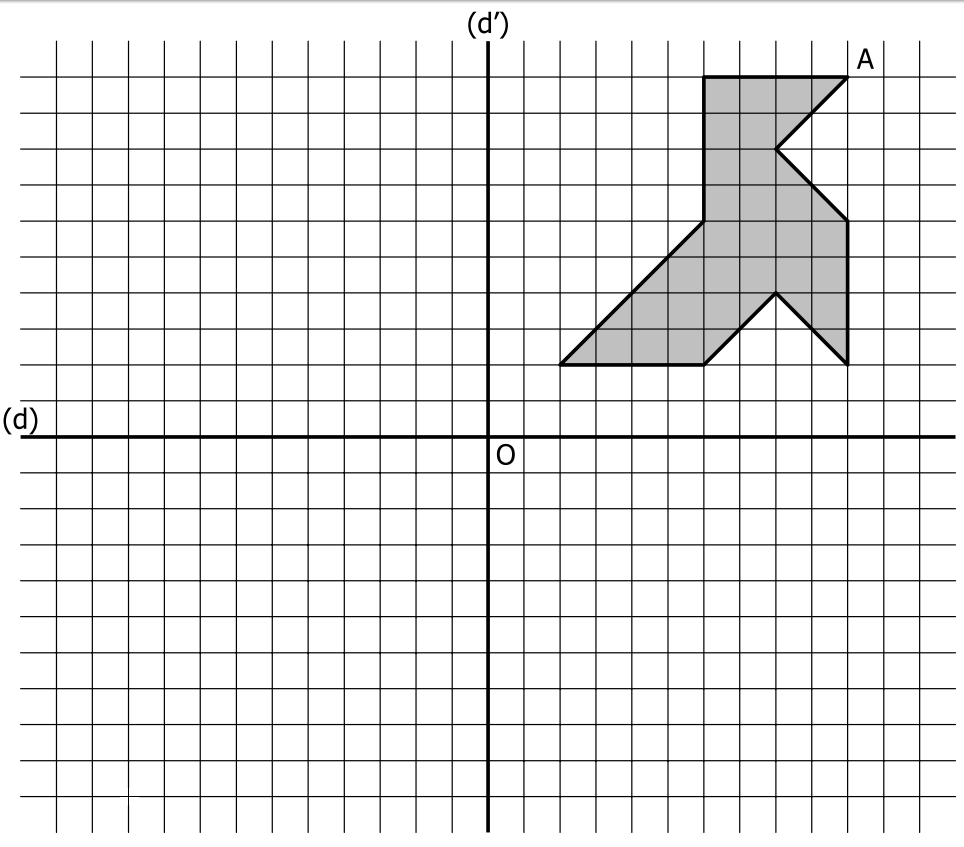
\includegraphics[scale=0.4]{img/fig2}
\end{center}


\section{Lire une figure (7 points)}

D'après la figure ci-dessous :

\begin{center}
	\includegraphics*[scale=0.25]{img/figure}	
\end{center}

\begin{questions}
	\question[1] Donner deux segments de même longueur.
	\begin{solution}
		Les segments $[CD]$ et $[GE]$ ont la même longueur. (ou $[AB]$ et $[BC]$, $[AG]$ et $[GE]$, $[AG]$ et $[GC]$, etc.)
	\end{solution}
	
	\question[1] Donner deux droites perpendiculaires.
	\begin{solution}
		Les droites $(AC)$ et $(AF)$ sont perpendiculaires.
	\end{solution}
	
	\question[1] Donner un segment et son milieu.
	\begin{solution}
		$B$ est le milieu de $[AC]$.
	\end{solution}
	
	\question[2] Citer tous les points situés à la même distance de $A$ que de $C$.
	\begin{solution}
		Les points $B$ et $G$ sont à la même distance de $A$ que de $C$ (on a $AB = BC$ et $AG=GC$)
	\end{solution}
	
	\question[2] Citer tous les points situés à la même distance de $C$ que de $E$.
	\begin{solution}
		Les points $G$, $H$ et $D$ sont à la même distance de $C$ que de $E$ (on a $GC = GE$, $HC=HE$ et $DC=DE$)
	\end{solution}
\end{questions}

\newpage
\section{Démonstrations (6 points)}

A partir de la figure ci-dessous :

\begin{center}
	\includegraphics*[scale=0.15]{img/figure2}	
\end{center}

\begin{questions}
	\question 
		\begin{parts}
			\part[1] Citer deux droites pour lesquelles on peut justifier qu'elles sont parallèles.
			\begin{solution}
				Les droites $(d_3)$ et $(d_4)$ sont parallèles.
			\end{solution}
			\part[2] Rédiger la démonstration.
			\begin{solution}
				\textbf{On sait que} $(d_3) \bot (d_2)$ et $(d_4) \bot (d_2)$.\\
				\textbf{Or} si deux droites sont parallèles à une même troisième droite, alors elles sont parallèles.\\
				\textbf{Donc} $(d_3) // (d_4)$.
			\end{solution}
		\end{parts}
	
	\question Dans cette question, on a : $(d_1) // (d_6)$
		\begin{parts}
			\part[1] Citer deux droites pour lesquelles on peut justifier qu'elles sont perpendiculaires.
			\begin{solution}
				Les droites $(d_6)$ et $(d_7)$ sont perpendiculaires.
			\end{solution}
			\part[2] Rédiger la démonstration.
			\begin{solution}
				\textbf{On sait que} $(d_1) \bot (d_7)$ et $(d_1) // (d_6)$.\\
				\textbf{Or} si deux droites sont parallèles , alors toute perpendiculaire à l'une est perpendiculaire à l'autre.\\
				\textbf{Donc} $(d_6) // (d_7)$.
			\end{solution}
		\end{parts}
\end{questions}


\section{Construction (6 points)}

\begin{questions}
	\question[3] Construire en vraie grandeur la figure ci-dessous.
	\begin{center}
		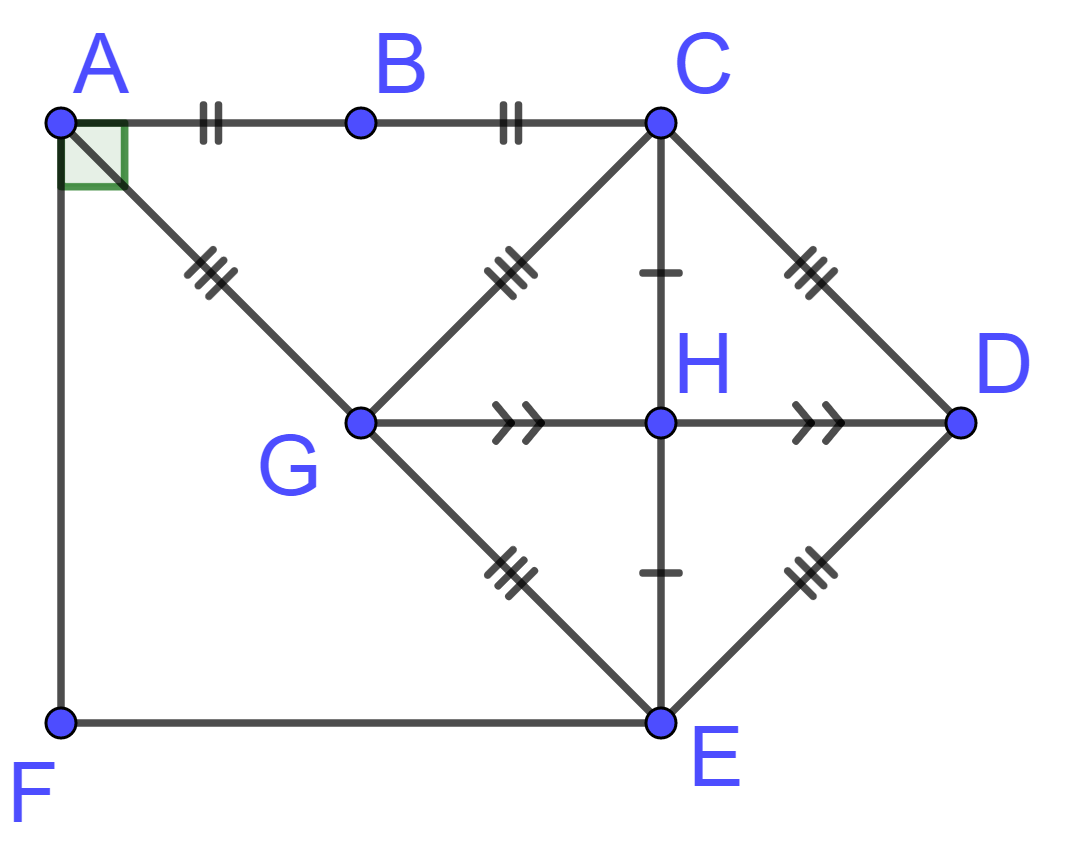
\includegraphics[scale=0.7]{img/figure}
	\end{center}

	\question 
		\begin{parts}
			\part[1] Sur votre figure, les points A, B et C semblent-t-ils alignés.
			
			\part[2] Le sont-ils vraiment ? Justifier votre réponse.
		\end{parts}
\end{questions}
\label{LastPage}

%\section{Consommation électrique}
%
%Une consommation d'électricité se mesure en 
\end{document}